\chapter{Verification, Evaluation, and Observability}
\label{ch:verification}

The complexity of distributed consensus makes manual verification impossible. This chapter details the multi-layered testing strategy employed to validate the system’s correctness, performance, and operational visibility.

Because distributed bugs can be hidden by race conditions and network delays, a robust evaluation strategy is required. This chapter covers the validation of consensus states through formal models, chaos engineering tests, and end-to-end integration traces.

\section{Correctness Testing}
\label{sec:correctness_testing}

To guarantee that the implementation adheres to the Raft specification, the project utilizes a comprehensive, multi-phase test suite that simulates the unpredictable nature of real-world networks. The testing framework focuses on three pillars: foundational protocol tests, end-to-end client cluster simulations, and formal linearizability verification.

\subsection{Foundational Testing: MIT 6.824 Methodology}
The core consensus logic is verified using an extensive test suite inspired by the MIT 6.824 Distributed Systems curriculum. These tests are divided into four sequential phases, covering both the consensus engine and the replicated state machine under various simulated network and crash conditions:

\begin{itemize}
    \item \textbf{Leader Election}: Tests such as \texttt{TestInitialElection} and \texttt{TestReelection} verify that a cluster successfully elects a single leader and maintains that leadership. Across multiple elections on reliable networks, the system achieves consensus with execution times ranging from 3.6 to 8.4 seconds, handling up to 954 operations.
    
    \item \textbf{Log Agreement}: Tests like \texttt{TestBasicAgree} and \texttt{TestFailAgree} ensure that the leader can correctly synchronize logs. The tests also cover situations where followers are temporarily offline, undergo progressive node failures, or possess conflicting entries. For example, edge cases—such as backing up quickly over incorrect follower logs—are handled with up to 1,528 RPCs executed within 12.1 seconds.
    
    \item \textbf{Persistence and Churn}: The \texttt{TestPersist} series validates that nodes resume operation after a crash without losing committed data. This includes Figure 8 edge-case validation and churn tests under unreliable networks, completing complex operations involving up to 7,204 RPCs in 16.1 seconds.
    
    \item \textbf{Log Compaction and Snapshotting}: Ensures that the log size stays reasonable. When followers fall too far behind, they are brought up to date using the \texttt{InstallSnapshot} RPC, successfully completing even during periods of network instability within 56.1 seconds.
\end{itemize}

\subsection{End-to-End Client Cluster Testing}
To demonstrate that the Raft engine properly interfaces with the Replicated State Machine and gRPC layers, end-to-end operations are tested under high load and adverse environments across clusters of 3, 5, and 7 nodes:

\begin{itemize}
    \item \textbf{Concurrent Operations and Load Balancing}: Tests execute sustained workloads of both read-only and write-heavy requests (e.g., many concurrent clients executing up to 3,247 requests in 3.9 seconds), validating leader hints and retries.
    
    \item \textbf{Network Partitioning and Healing}: The cluster accurately prevents writes to the minority partition during split-brain scenarios and resumes completion once healed.
    
    \item \textbf{Randomized Keys and Failures}: Long-duration runs combining randomized keys, server crashes, and network partitions (over 12.1 seconds) confirm that system liveness and linearizability are retained.
\end{itemize}

\subsection{Chaos Simulation and Unreliable Networks}
To simulate the "adversarial" nature of distributed environments, the project implements a custom \texttt{Network} simulator located in the \texttt{testutils} package. This simulator allows the test suite to programmatically induce network failures:

\begin{itemize}
    \item \textbf{Network Partitions}: Nodes are split into isolated groups (e.g., a 3-node majority and a 2-node minority) to verify that the system remains linearizable.
    \item \textbf{Packet Loss and Delays}: RPCs are randomly dropped or delayed to ensure the consensus engine is robust against high latency and message reordering.
    \item \textbf{Server Crashes}: Nodes are abruptly killed and restarted during active replication to verify the durability of the state machine.
\end{itemize}

The chaos engine operates concurrently with the client. This "stress testing" ensures that edge cases—such as a leader failing exactly at the moment of commitment—are correctly handled without data loss.

\subsection{Linearizability Verification with Porcupine}
While standard tests check for specific failure modes, they cannot prove that every execution trace is linearizable under concurrent client access. To achieve this, the project integrates the \textbf{Porcupine} linearizability checker, an efficient implementation of a linearizability checker designed specifically for testing distributed systems in Go.

\paragraph{Why Linearizability Matters}
Linearizability ensures that every operation appears to take effect atomically at some point between its invocation and its response, creating a single, globally ordered timeline. In an asynchronous environment, concurrent client requests and leader elections can introduce reordering or stale reads if the consensus implementation contains subtle bugs. Porcupine detects these anomalies by validating execution traces against a strict sequential consistency model.

\paragraph{Verification Methodology}
The verification process follows three steps:
\begin{enumerate}
    \item \textbf{Trace Logging}: During chaos tests, the system records every request's start time, end time, and result (invocation and response).
    \item \textbf{Model Definition}: A formal model of a sequential key-value store is provided to Porcupine, defining the expected output for every \texttt{Get} and \texttt{Put} operation.
    \item \textbf{Trace Validation}: Porcupine analyzes the concurrent logs to determine if there exists a valid sequential execution that respects the real-time ordering of the operations.
\end{enumerate}

Porcupine is important to the correctness argument of this thesis because it explores the state space of concurrent operations. It verifies that even under severe network partitions and concurrent recoveries, the cluster does not yield stale or out-of-order data.

\begin{table}[h]
\centering
\caption{Results of Chaos and Linearizability Stress Tests.}
\label{tab:test_results}
\begin{tabular}{|l|l|l|l|}
\hline
\textbf{Test Category} & \textbf{Nodes} & \textbf{Chaos Type} & \textbf{Status} \\ \hline
MIT Raft Suite & 3--5 & Re-elections, Partitions & PASS \\ \hline
KV E2E Stress & 5 & Concurrent Put/Get + Restarts & PASS \\ \hline
Linearizability Chaos & 5 & Partitions + Server Crashes & PASS \\ \hline
Snapshot Stress & 3 & High-load with Compaction & PASS \\ \hline
\end{tabular}
\end{table}

The status summarized in Table \ref{tab:test_results} confirms that the implementation maintains strict consistency. By passing the Porcupine verification even under severe network partitions, we demonstrate that the "strong leader" and "quorum commitment" logic correctly implement the linearizable consistency model required for a reliable distributed state machine.

% \section{Performance Analysis}
% \label{sec:performance_analysis}
% To evaluate the efficiency of the implementation, a series of benchmarks were conducted focusing on latency, throughput, and recovery speed. These tests were performed using the automated deployment framework on a 5-node cluster.

% \subsection{Latency Comparisons: 3 vs. 5 Nodes}
% The latency of a \texttt{Put} operation is directly affected by the number of nodes in the cluster, as the leader must wait for a majority to acknowledge the entry before committing. 

% \begin{table}[h]
% \centering
% \caption{Average latency for a \texttt{Put} operation across different cluster sizes.}
% \label{tab:latency_comparison}
% \begin{tabular}{|l|l|l|}
% \hline
% \textbf{Cluster Size} & \textbf{Quorum Size} & \textbf{Avg. Latency (ms)} \\ \hline
% 3 Nodes & 2 Nodes & [Value] ms \\ \hline
% 5 Nodes & 3 Nodes & [Value] ms \\ \hline
% \end{tabular}
% \end{table}

% As shown in Table \ref{tab:latency_comparison}, increasing the cluster size from 3 to 5 nodes typically results in a slight increase in latency. This is expected behavior in Raft, as the leader must wait for responses from more followers to satisfy the quorum requirement. However, the 5-node cluster provides higher fault tolerance, surviving the simultaneous failure of two nodes.



% \subsection{Throughput: Read-Heavy vs. Write-Heavy Workloads}
% Throughput was measured by executing a sustained volume of operations. The system's performance varies significantly based on the ratio of \texttt{Get} to \texttt{Put} requests.

% \begin{itemize}
%     \item \textbf{Write-Heavy (80\% Put)}: Performance is limited by the I/O bottleneck of persisting logs to disk and the network round-trip time required for consensus.
%     \item \textbf{Read-Heavy (80\% Get)}: While reads in this implementation still pass through the Raft log to ensure strict linearizability, they generally exhibit lower latency than writes because the state machine does not need to update its persistent version.
% \end{itemize}



% \subsection{Recovery Time Analysis}
% A critical metric for a high-availability system is the time required to resume normal operation after a leader crash. This depends on the detection of the failure via heartbeat timeouts and the completion of a new election.

% The recovery process is governed by the \texttt{electionTimer} settings in the configuration.
% By tuning the \texttt{RAFT\_ELECTION\_TIMEOUT\_MIN} and \texttt{RAFT\_ELECTION\_TIMEOUT\_RAND} parameters, the system can balance between rapid failure detection and the risk of frequent unnecessary elections due to network jitter.

\section{Observability and Metrics}
\label{sec:observability}
The system integrates a modern monitoring stack to provide real-time insights into the distributed state. This is achieved through the combination of Prometheus for metrics, Loki for logs, and Grafana for visualization.

Operators can use these metrics to monitor replication latency and ensure the cluster maintains progress during heavy workloads or network partitions. This observability layer helps debug state issues in real time.

\subsection{Metric Collection with Prometheus}
Each node exports instrumentation data that is periodically scraped by Prometheus, providing deep visibility into the consensus runtime. This allows for the tracking of critical consensus invariants and state machine execution:
\begin{itemize}
    \item \textbf{Commit and Application Progress}: The \texttt{raft\_commit\_index} and \texttt{raft\_last\_applied} gauges allow operators to monitor replication lag. A widening gap between the commit index and the last applied index indicates that the node's applier goroutine is lagging behind the consensus layer.
    
    \item \textbf{Cluster Logical Time}: The \texttt{raft\_current\_term} gauge tracks the current logical term of the node. Monitoring this metric helps detect rapid term changes or unstable elections, which can point to underlying network partitions or split-brain scenarios.
    
    \item \textbf{Leadership Transitions}: The \texttt{raft\_leader\_changes\_total} counter provides a history of term changes, which is vital for diagnosing cluster instability. Frequent leadership transitions under heavy workloads indicate that election timeouts require adjustment to prevent network jitter.
    
    \item \textbf{Node State Tracking}: The \texttt{raft\_state} gauge (0=Follower, 1=Candidate, 2=Leader) provides an instant, real-time view of the cluster topology. This helps operators ensure that the cluster has an active, single leader.
    
    \item \textbf{Workload and Throughput}: The \texttt{raft\_client\_requests\_total} counter records the total volume of \texttt{Put} and \texttt{Get} operations processed by the cluster, which allows operators to correlate performance spikes with system throughput.
\end{itemize}

\subsection{Log Aggregation with Loki and Visualization in Grafana}
Structured logs produced by the \texttt{zap} logger are ingested by Promtail and forwarded to Loki.
This centralized log repository enables searching for specific request IDs or terms across the entire cluster.
As seen in the integrated dashboards in Figure \ref{fig:grafana_dashboard}, these tools provide a comprehensive "control room" for the distributed system, allowing operators to verify that the cluster makes safe, quorum-based decisions.

\begin{figure}[htbp]
    \centering
    \begin{subfigure}[b]{1\textwidth}
        \centering
        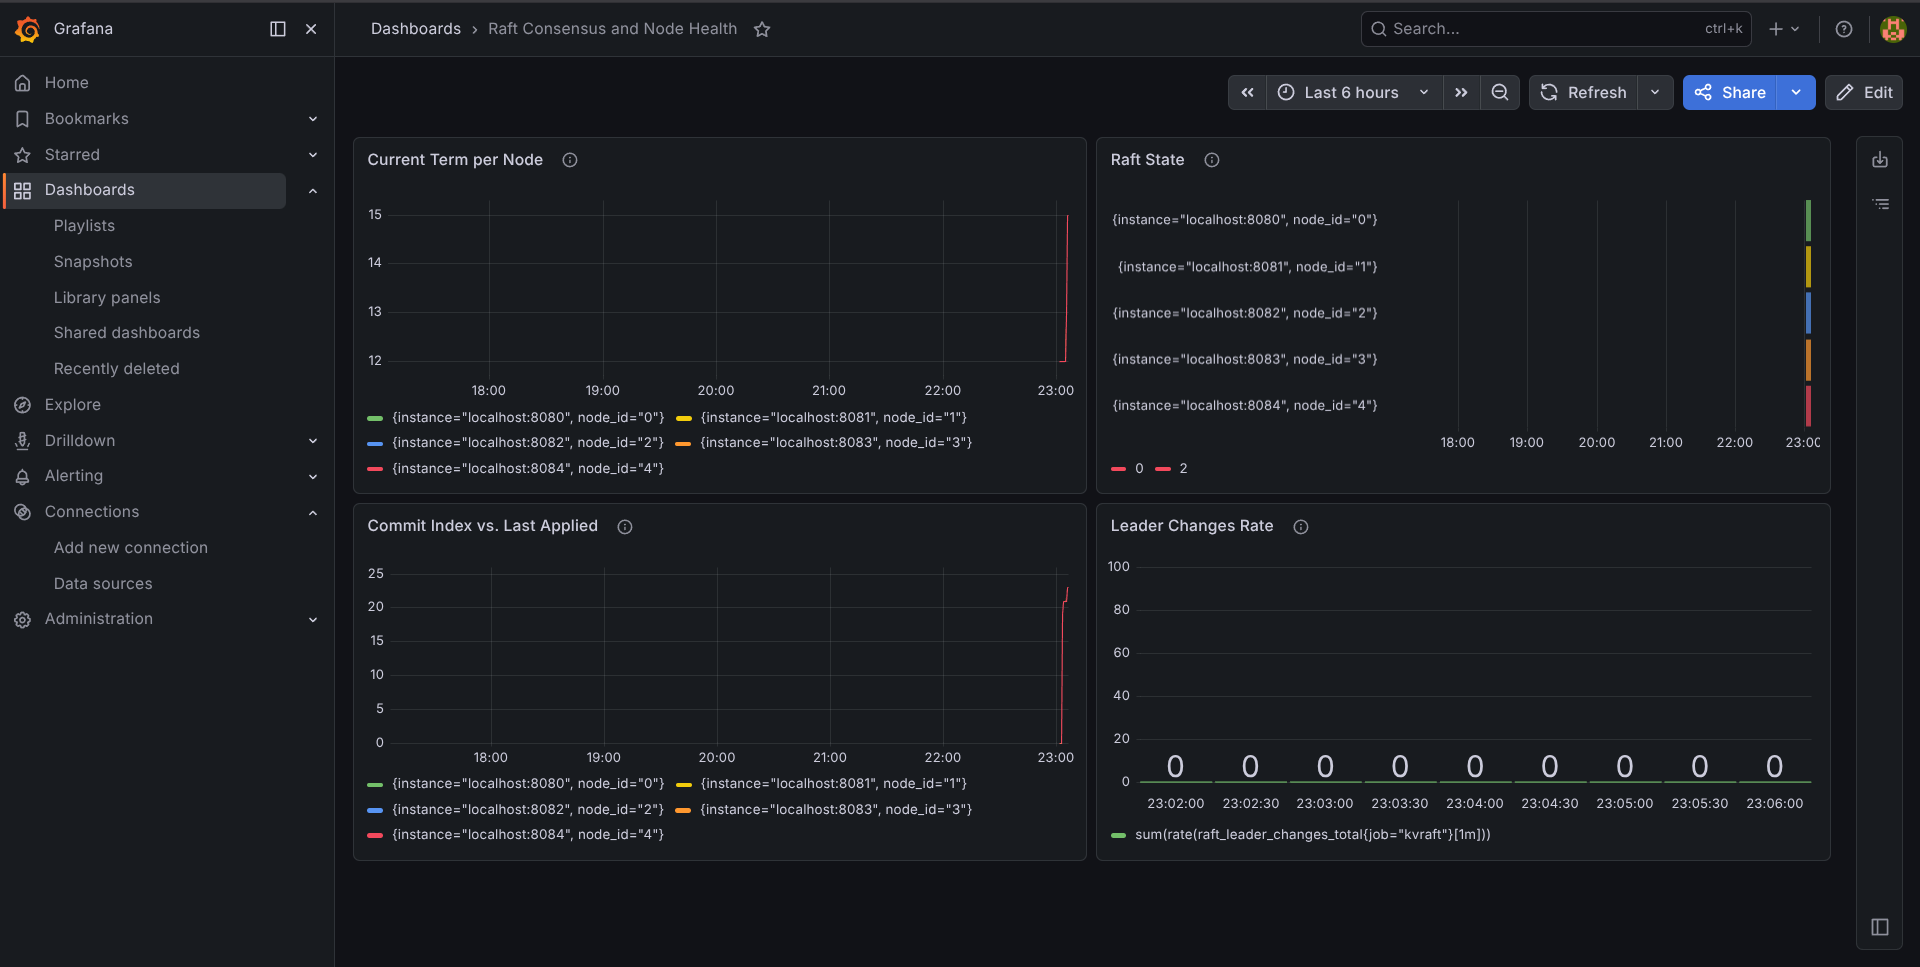
\includegraphics[width=\textwidth]{figures/prometheus.png}
        \caption{Prometheus metric collection}
        \label{fig:prometheus_metrics}
    \end{subfigure}
    
    \vspace{1em} % Adjust the vertical space between subfigures
    
    \begin{subfigure}[b]{1\textwidth}
        \centering
        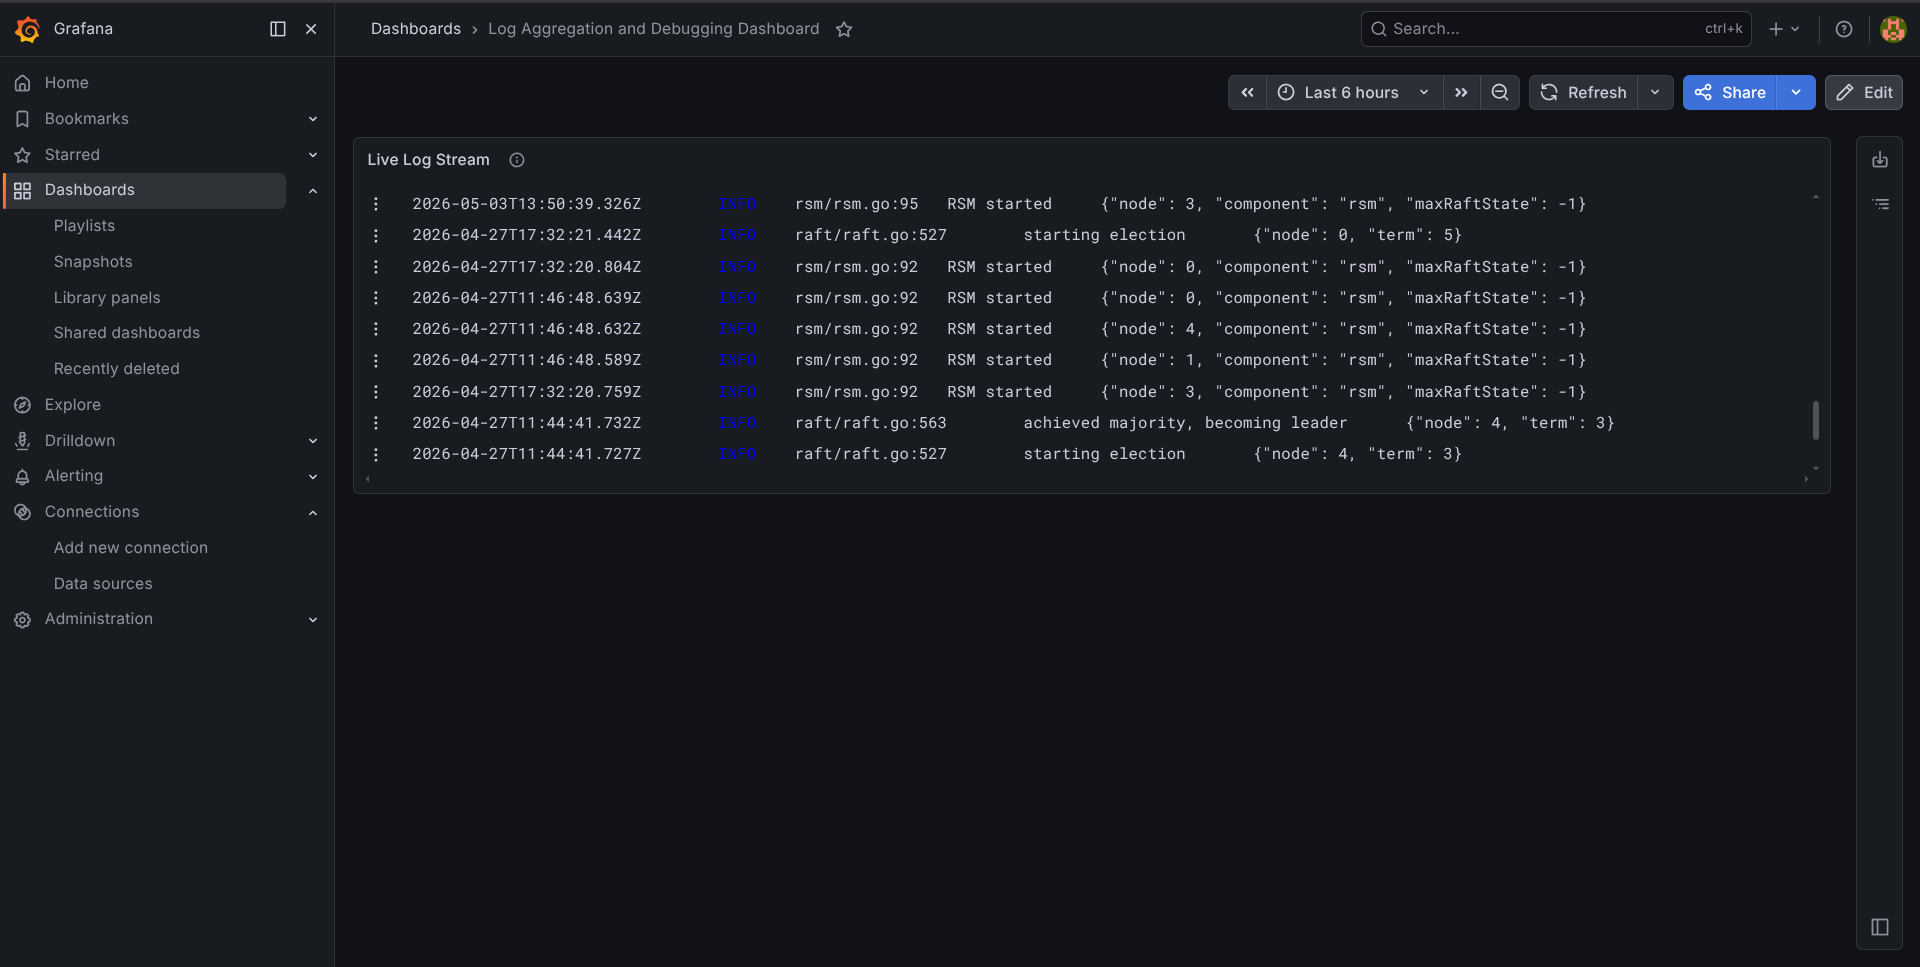
\includegraphics[width=\textwidth]{figures/loki.png}
        \caption{Log aggregation in Loki}
        \label{fig:loki_logs}
    \end{subfigure}
    \caption{Integrated Grafana observability dashboards for the distributed system.}
    \label{fig:grafana_dashboard}
\end{figure}

By correlating metrics and logs, we can verify that the system is functioning as intended, such as ensuring that the \texttt{commitIndex} only advances when a majority of nodes have acknowledged the data.